\documentclass[12pt, oneside]{extbook}

\usepackage{geometry}
\usepackage{graphicx}
\usepackage{listings}
\usepackage[dvipsnames]{xcolor}
\usepackage[italian]{babel}
\usepackage{amssymb}
\usepackage{mathrsfs}

\geometry{
	a4paper, 
	top = 2cm,
	left = 1.5cm,
	right = 1.5cm,
	bottom=2cm
}
\lstset{
	language=Python, 
	%frame=shadowbox,
	%rulesepcolor=\color{gray!50},
	basicstyle=\ttfamily\small,
	keywordstyle=\color{purple}\bfseries\small,
	stringstyle=\color{ForestGreen}\small,
	commentstyle=\color{blue}\small,
	numbers=left,
	numberstyle=\small\color{black},
	numbersep=5pt,
	tabsize=2,
	showtabs=false,
	showspaces=false,
	showstringspaces=false,
	%escapechar=|,
	%captionpos=b,
	breaklines=true,
	keepspaces=true
}

\title{Machine Learning}
\author{Pierciro Caliandro}

\begin{document}
\maketitle
\tableofcontents
\chapter{Introduzione del corso}
\section{Introduzione}
Per il progetto: sviluppare	un notebook in cui la parte espositiva sia presente, quindi intercalare markdown + codice, dove il markdown deve esserci e deve essere eloquente.\\NON solo codice, esporre i ragionamenti, le limitazioni etc...\\
\section{Presentazione del ML}
L'informatica è risolvere problemi da un punto di vista algoritmico, risolvere un problema attraverso algoritmi si può dividere in fasi:
\begin{itemize}
	\item analizzare il problema
	\item vederlo in modo matematico
	\item pensare ad un algoritmo
	\item implementarlo in un linguaggio
	\item verificare la correttezza (attività di testing) e valutarne l'efficienza
\end{itemize}
Il caso elementare può essere un testo dove si richiede di trovare i caratteri i nel testo: l'algoritmo può scorrere un carattere alla volta e contare ogni i. L'algoritmo funziona sulla base di un assunto, ovvero che sappiamo riconoscere la i, quindi che l'algoritmo sappia cosa è una i o cosa non lo sia, quindi abbiamo bisogno di una definizione del carattere che permetta alle persone di riconoscere il carattere.\\Possiamo dare varie definizioni:
\begin{itemize}
	\item riconoscere la i come na' sbarretta co' un puntino sopra
	\item sequenza ASCII, UNICODE, ovvero una sequenza di bit
\end{itemize}
A volte non è facile: il problema può essere simile ma in un contesto diverso, ovvero ad esempio se occorre riconoscere quante volte in una sequenza di foto compaia una certa persona (NDR: Emma Stone, bello sticchio).\\Il metodo che si applica può essere triviale e non può essere codificato, come ad esempio riconoscere una faccia o capire un testo parlato.\\Non abbiamo quindi una chiara definizione di cosa cerchiamo di identificare, quindi come facciamo a definirla: una caratterizzazione di una persona per attributi è un po' complicata e non esaustiva. Se non possiamo fare così, possiamo farlo per esempi: forniamo una serie di foto di quella persona, non siamo in grado di definirla formalmente, possiamo poi dare degli esempi di foto che non ritraggono quella persona. Ci si muove quindi in modo induttivo, caratterizzando sulla base di singoli specifici esempi, in ML si cerca di fare questo: problemi per cui non si riesce a fornire una soluzione in quanto troppo complessi si prova a risolverli a partire da esempi.\\Entra in gioco l'induzione, quindi non so riconoscere la persona ma posso mostrare solo degli esempi e quindi potrò avere un algoritmo derivato dall'insieme di esempi, tale per cui sottoponendo una foto questo ci dice se è della persona o meno con una certa precisione.\\Quindi, nel ML, \textbf{a partire dai dati vogliamo derivare un algoritmo che ci dia delle perdizioni}, per poter derivare un algoritmo serve un altro algoritmo.\\Abbiamo quindi:
\begin{itemize}
	\item i dati
	\item l'algoritmo da derivare
	\item l'altro algoritmo, che è un \textbf{sistema o modello di ML}
\end{itemize}
Vorremmo quindi un algoritmo che \textbf{apprenda} come fare una cosa, che è un modo accorciato perché in realtà l'algoritmo sulla base dei dati, ne produce un altro per rispondere ad una domanda ben precisa.\\Un esempio classico è considerare il problema in contesti più complessi come ad esempio riconoscere un carattere scritto a mano: è l'"Hello World" del ML, dove abbiamo dei caratteri scritti a mano (delle immagini), da cui voglio ottenere un algoritmo che sia in grado di riconoscere la cifra corrispondente, sulla base di esempi che sono la coppia $<$ immagine, cifra corrispondente $>$, come nel caso precedente della classificazione di persone.\\È in questo caso una classificazione \textbf{multiclasse}, ma come prima abbiamo un elemento per cui abbiamo la risposta corretta, da cui vogliamo realizzare un sistema per cui la risposta corretta non c'è ma deve essere probabilmente corretta.\\Normalmente a grandi linee, un sistema di ML cosa fa:
\begin{itemize}
	\item costruisce un modello, l'informazione va trattata da algoritmi e quindi va formalizzata matematicamente.\\Si costruisce ad esempio un range 0-9, abbiamo per esempio immagini 28x28 in scale di grigi, abbiamo quindi un vettore di 28x28 = 784 valori, ognuno è un intero compreso fra 0, 255. Un elemento è quindi un punto in uno spazio di 784 dimensioni
	\item geometricamente, l'insieme di tutti i caratteri è un insieme di punti in uno spazio a 784 dimensioni, vorremmo ottenere un modo per tagliare lo spazio in modo che da una parte ci siano solo 0, da una solo 1 e così via... generando così delle zone associata ad un singolo valore così che qualunque punto che cade in una zona è associato ad un certo valore
	\item in altro modo, vogliamo una funzione f da \{0,1,...,255\}$^{784}$ in \{0,1,2...,9\}
	\item in realtà definiamo un funzione per ogni carattere, ognuna di esse data un'immagine che è un vettore, restituisce un valore che è una probabilità che l'elemento sia 0,1.... così da poter associare tale elemento al valore in base a quale ha la probabilità più alta.\\Devono ovviamente valere tutte le ipotesi per le funzioni di densità
\end{itemize}
A partire dai dati cerchiamo quindi delle funzioni, ma la cerchiamo in un insieme di funzioni e tale funzione cercata deve essere tale per cui va dal dominio di interesse al codominio di interesse. Ci saranno un infinità di funzioni di questo tipo, ma ne devo determinare una: prendo la funzione che, se le faccio fare le previsioni per gli elementi di cui so già la risposta, vorrei che questa faccia il minor numero di errori possibile.\\So la risposta giusta, cerco fra un campione della popolazione delle funzioni per cercare la migliore, quindi occorre avere intanto un \textbf{costo}, ovvero quanto sta sbagliando la funzione:
\begin{itemize}
	\item potrei vedere quante volte sbaglia
	\item ci possono essere metodi diversi, ma c'è sempre un'idea di costo
\end{itemize}
Fra tutte le funzioni, si prende quella il cui costo sui dati è il più piccolo possibile.\\Tutte le possibili funzioni? Sono infinite, quindi quello che si fa è considerare tutte le funzioni che hanno la stessa struttura, ad esempio che sono lineari o quadratiche: se ad esempio sono tutte lineari, la funzione farà una combinazione lineare dei valori e produrrà l'output. Avrò quindi una \textbf{struttura} che definirà delle funzioni che differiscono in base ai parametri, quindi cerchiamo la migliore funzioni e quindi il miglior vettore di parametri che corrisponde alla funzione che si comporta meglio.\\Passiamo quindi da una ricerca di funzioni ad una in uno spazio di parametri, quindi minimizziamo qui.\\Le funzioni nella classe saranno quindi caratterizzati dai valori dei parametri, similmente avviene in statistica: se abbiamo un insieme di elementi e vogliamo dargli una rappresentazione statistica, consideriamo magari una distribuzione Gaussiana cercando quella che rappresenta meglio l'insieme, quindi cambieranno media e varianza.\\Passiamo da ottimizzazione su funzioni ad ottimizzazione su parametri.\\Stiamo facendo un'ipotesi, che può comunque essere sbagliata, ma nel momento in cui facciamo un'ipotesi cerchiamo la funzione migliore che sarà quella che "farà meno errori", in relazione al come io caratterizzo gli errori.\\Un concetto importante è la \textbf{funzione di costo}, ovvero il modo in cui conto gli errori, che sarà quella che devo minimizzare.\\Questa è l'impostazione del \textbf{supervised learning}: prediciamo un valore per un elemento sulla base di un insieme di elementi dati. A sua volta, si dividerà in varie classi (non le riporto ora perché tanto le riprendiamo più avanti).
	

\chapter{Fondamenti del ML}
\paragraph{Approccio induttivo}
Nel ML, a differenza dello sviluppo di algoritmi tradizionale, si usa un approccio induttivo, in quanto abbiamo difficoltà nel precisare i passi da attuare per risolvere un problema di predizione.\\L'idea è muoversi sulla base del tentativo di apprendere dei \textbf{pattern} sulla base di un inseme di esempi: cerchiamo di apprendere delle caratteristiche comuni ad un inseme di esempi sottoposti all'algoritmo. Siamo ad un livello "meta": l'algoritmo fornirà a sua volta un algoritmo.\\Assumiamo di avere a disposizione un insieme di esempi che è il training set, tipicamente assumeremo che ognuno degli esempi sia rappresentato da un vettore di valori, quindi n vettori $x_1$, ..., $x_n$ di stessa dimensione d, quindi un elemento è rappresentato da d valori reali o interi.\\Ognuno di questi d valori è associato a qualche caratteristica, quindi ogni elemento del mondo considerato è rappresentato attraverso d sue caratteristiche numeriche.\\Es: abbiamo un insieme di persone e voglio predire il sesso sulla base di peso ed altezza. Ogni persona sarà rappresentata con i valori di queste due caratteristiche, che sono le \textbf{features} e sono tutto quello che assumo di conoscere e tutta l'informazione per effettuare la predizione.\\Mi aspetto di avere vettori bidimensionali di 2 componenti, nel training set associato ad ognuno dei valori c'è il sesso associato alla persona, c'è anche il valore della variabile da predire.\\Il valore da predire prende il nome di \textbf{target}, il sistema deve quindi essere in grado di: preso un insieme di vettori di 2 dimensioni, ognuno col il valore del target, vogliamo un metodo per derivare un altro metodo che a partire dalle feature mi dica se la persona è maschio o femmina, con una buona precisione.\\Dobbiamo avere una valutazione di quanto si comporta bene il metodo, va quindi sperimentato su dei dati, ad esempio vedendo quante volte sbaglia ma qual è l'insieme dei dati? Cosa vuol dire "quanto sbaglia"? Serve una funzione di errore.\\Abbiamo lo schema seguente:\\
\begin{figure}[!h]
	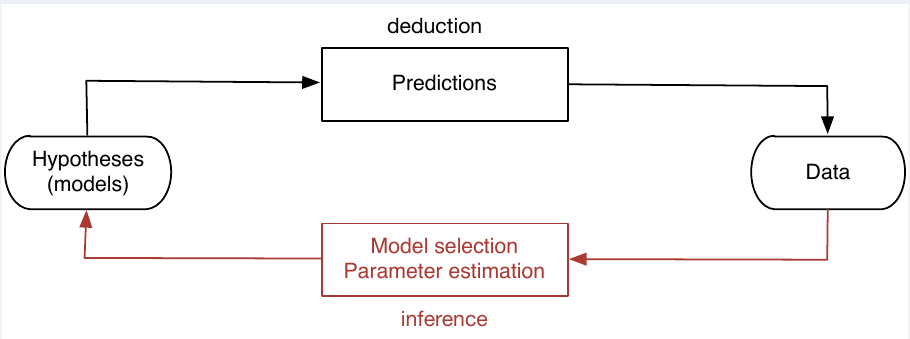
\includegraphics[scale=0.5]{immagini/schema-modello.png}
	\caption{Schema generale della derivazione di un modello di ML}
\end{figure}\\
l'algoritmo di predizione viene chiamato in ML \textbf{modello}. Il processo è tipicamente iterativo: a partire dai dati si fa un ipotesi su come è fatto il modello, si misurano le prestazioni ed eventualmente si migliora il modello in qualche modo.\\\\
\paragraph{Supervised learning}
Quello di cui stiamo parlando è il supervised learning: il training set è un insieme di vettori con un valore target associato ad ogni elemento, sarà una matrice X, con dimensione nxd, per ognuno degli elementi ci sarà il vettore target di n elementi.\\Geometricamente è come se avessi un insieme di n punti in uno spazio di d dimensioni ed a cui è associato un valore, voglio quindi trovare un modo per dividere lo spazio di d dimensioni: sempre nel caso sesso vs altezza, peso, gli elementi saranno punti in uno spazio 2D, alcuni maschi e femmine. Vorrei avere un metodo, ovvero una decomposizione dello spazio in regioni in cui ad ogni regione associo un valore del target così che quanto arriva un nuovo elemento, in base alla regione dove cade so il valore del target.\\Partiziono quindi lo spazio del dominio D in regioni, è solo un modo diverso di vedere la cosa.\\Abbiamo poi un'ulteriore divisione, in base al fatto che il valore target sia reale o discreto:
\begin{itemize}
	\item nel primo caso si parla di \textbf{regressione}: ho un inseme di caratteristiche su un immobile, a partire dal quale voglio conoscere il valore sul mercato
	\item parlo altrimenti di classificazione, nel caso in cui il numero di classi sia finito, come nel caso della perdizione M/F (classificazione binaria)
\end{itemize}
A questo punto, abbiamo il training set e vogliamo dedurre come poter predirre il target a partire dalle feature, anche qui abbiamo una divisione:
\begin{itemize}
	\item cerchiamo di ottenere una funzione $y()$, che ha come dominio un vettore di feature e restituisce un codominio: y: $\mathbb{R} \rightarrow \mathbb{R}$, arriva un $x$ di cui non conosco il target e faccio $y(x)$
	\item approccio probabilistico in cui cerchiamo di ottenere una distribuzione di probabilità per ognuno degli elementi, a partire dalla sue feature. Tale distribuzione sarà su tutti i valori del target.\\Pensando all'esempio di prima, la persone è alta 1.68 e pesa 57kg, l'algoritmo deve dirmi che col 73\% è femmina e col 100-73 è maschio. Questo caso è molto più informativo del primo, possiamo anche stimare meglio l'affidabilità che è legata in qualche modo alla varianza della distribuzione.\\Inoltre, se il sistema da una distribuzione di probabilità dei possibili valori target, dire Maschio/Femmina serve un metodo che stabilisce effettivamente il valore target da assegnare (serve quindi un passo in più).\\Magari non conviene semplicemente assegnare in base alla probabilità più alta, ad esempio quando gli errori non pesano allo stesso modo: se prendiamo l'esempio del covid, se il sistema è probabilistico ci saranno degli errori che sono falsi positivi o falsi negativi.\\In questo contesto i due errori non pesano allo stesso modo.\\C'è un discorso che ha quindi a che fare con la gestione del rischio, che rende possibile l'attuazione di politiche ulteriori e quindi rende questo approccio più informativo del primo
\end{itemize}
\paragraph{Unsupervised learning}
Qui non abbiamo il valore del terget, quindi il problema non è prevedere il valore del target ma: ho un insieme di valori di elementi e in qualche modo voglio riuscire ad estrarre dell'informazione che viene rappresentata da quell'insieme di elementi.\\Supponiamo di avere elementi in uno spazio 2D, dall'osservazione del dataset possiamo stabilire due cose (metti magari disegno):
\begin{itemize}
	\item il fatto che gli elementi possono raggrupparsi in gruppi abbastanza separati fra loro. Possiamo osservare la tendenza a raggrupparsi in così detti \textbf{cluster} un analisi che cerca di capire se avviene tale raggruppamento è il \textbf{clustering}.\\Un esempio è cercare ad esempio di raggruppare in un certo numero di cluster, vedere in quanti cluster sta uno stesso elemento, l'idea è dire che gli elementi si raggruppano in qualche modo per via di una certa variabile che non vediamo e determina tale raggruppamento.
	\item possiamo osservare che gli elementi non sono completamente sparsi su tutto il dominio, ma sono introno ad una retta, gli elementi più o meno sono intorno lì.\\Quindi i valori delle feature stanno più o meno intorno ad uno spazio di dimensione 1.\\C'è quindi una regolarità in quanto le i valori delle feature non sono totalmente indipendenti fra loro, la variabile è quindi una sola e che determina la posizione del punto sulla retta. L'idea è che le feature con cui rappresentiamo gli elementi non sono fra loro indipendenti, quindi in realtà i gradi di libertà veri sono di meno rispetto al numero di feature considerate.\\Potremo avere una situazione in cui i punti non sono proprio sulla retta ma intorno ad essa, il che vuol dire che le feature dipendono anche da altro e non da una sola variabile.\\Questo si chiama \textbf{feature selection} o \textbf{feature extraction}.\\Caso limite: dei punti che hanno tutti la stessa valore della y e diversi della x, andiamo quindi ad estrarre un sotto insieme dalle feature ottenendo dei vettori di dimensione $d'< d$.
	\item selezione di outlayers: un outlayer è un valore molto distante da tutti gli altri, ad esempio quando si fa analisi di log cerchiamo di trovare outlayers. \textsf{\textbf{un nero in Cina e misuri il suo bel cazzone e quello degli altri (l'ha scritto Gian Marco)}}. Definiamo una distribuzione di probabilità sui dati, per poi verificare la probabilità di ciascun elemento, se tale probabilità è bassa vuol dire che il punto è "strano" 
\end{itemize}
\paragraph{Reinforcement learning}
Apprendimento in cui ciò che vogliamo apprendere non è: consideriamo il caso supervisionato come raffronto, nel cui caso vogliamo predirre il valore del target.\\In questo caso vogliamo tirare fuori un algoritmo, una serie di passi che possono essere eseguiti: un esempio tipico è l'apprendimento automatico del movimento del drone, quindi a guida autonoma. Non è possibile elencare cosa fare in corrispondenza ad ogni singolo evento, ma si porta il sistema in cui ogni cosa avviene, in corrispondenza in cui ogni cosa che accade l'algoritmo deve prendere una decisione per poi massimizzare (una funzione?? Bho, non lo approfondiremo).\\Ha a che fare con tutti i sistemi che operano nel tempo.\\C'è una funzione di premio o penality per ogni possibile stato: il sistema quando parte prova a vedere dove va a finire ed apprende che una certa sequenza di mosse porta ad una situazione vantaggiosa o svantaggiosa\\\\

Siamo nel caso supervisionato: abbiamo quindi un insieme di possibili valori, il dominio $\mathscr{X}$ che è l'insieme degli oggetti che vorremmo poter etichettare. Ogni oggetto è modellato con un vettore di feature, intendiamo:
\begin{itemize}
	\item dimensione è la grandezza del vettore di feature.
	\item il numero di fetaure è la dimensionalità
\end{itemize}
L'insieme delle label è $\mathscr{Y}$, il training set è una matrice $\mathscr{X}$ in cui le righe corrispondono ai vettori di feature ed il target è un vettore colonna.\\Tutto ciò che diremo parte da un modello generale della situazione: abbiamo un insieme di dati che è il tranining set, che sarà quindi un campione (in termini statistici), quindi assumiamo che tali oggetti rappresentino un campione sul dominio dei possibili valori.\\Avremo quindi il training set 
$\mathscr{T}$ = \{(\textbf{x$_1$}, t$_1$),...,(\textbf{x$_n$}, t$_n$)\}.\\Denoteremo poi con \textbf{X} la matrice delle feature:\\
\textbf{X} = 
\\L'estrazione sarà avvenuta usando una qualche distribuzione di probabilità che non conosciamo, che è la distribuzione degli elementi ed è come aver preso a caso gli elementi secondo tale distribuzione, quindi la probabilità di prendere l'elemento è proprio secondo quella della distribuzione.\\Quindi $\forall x, p_{D_1}(x)$ è la probabilità di estrarre x data la distribuzione D.\\Per la label: supponiamo di aver estratto x secondo $D_1$, allora il target relativo verrà estratto da un urna dove ci sono tutti i valori target, con una distribuzione di probabilità $D_2$ che sarà però condizionata ad X, quindi $p(t|x)$.\\Assumiamo quindi di avere $D_1$, $D_2$ che è condizionata, di aver preso le feature x da $D_1$ e per ognuno di essi di aver estratto la label da $D_2$: $p_{D_2}(t|x)$.\\Supponiamo di avere $x \in X$, questo x ha una sula label corretta che chiamiamo y.Supponiamo di fissare un predittore, ovvero (in questo caso) una funzione $h$ che preso x fornisce una previsione. Possiamo fare $h(x)$ e confrontare il valore predetto con quello corretto e stabilire l'errore che sto facendo (ovvero un \textbf{NUMERELLO}). Possiamo fare questo confronto nel training set, per stabilire quanto sto sbagliando usiamo una funzione predefinita, da yxy $\rightarrow$ R, che chiamo \textbf{funzione costo}, $L(h(x), y)$. Più sarà elevato il valore dato dalla funzione loss e più stiamo sbagliando, consideriamo tutto come funzione di h: fissato il punto, cambiando h otteniamo una previsione diversa e quindi un valore diverso di loss per cui voglio scegliere la h tale per cui il valore di errore sia il più piccolo possibile.\\Il punto rimane fisso, vario $h$ e scelgo quella con loss migliore e questa è l'ottimizzazione.\\Il \textbf{rischio della predizione} è il valore della funzione loss, ovvero il rischio che ci si assume nel fare la predizione $h(x)$ invece di y.\\Il problema è trovare, di tutte le funzioni di predizione quella "buona" e non basta considerare solo un punto, occorre sceglierne una che tenda a comportarsi bene per tutti i punti, ovvero una per cui \textbf{la media del rischio} è più bassa possibile, in modo che se estraggo punti a caso e la media è la più bassa, la funzione può essere quella buona:
\begin{equation}
	R(y', x) = E_ {D_2}[L(y', y)] = \int\limits_{Y} L(y', y) \cdot p_{D_2}(y|x) dy
\end{equation}
oppure nel caso discreto
\begin{equation}
	R(y', x) = E_ {D_2}[L(y', y)] = \sum\limits_{Y} L(y', y) \cdot p_{D_2}(y|x)
\end{equation}	
dove L(y', y) è il costo nel caso in cui il valore target è quello e la previsione è quella che fa la $h(y)$ (sarebbe il valore di loss).\\La predizione ottima, in questo caso, è quella per cui il rischio è il più basso possibile: arriva x, supponiamo che la label sia M/F. Una politica è dire che, se rispondo M ed è M abbiamo un certo valore della loss, ma abbiamo anche una certa probabilità associata che magari è bassa. Nel caso F, abbiamo del rischio ma associato alla probabilità più alta. Consideriamo quindi la somma delle due cose, rispondendo sempre la cosa che fa minimizzare il rischio e quindi 
\begin{equation}
	argmin_{y} R(y', x)
\end{equation}
quanto io sbaglio dipende dal rischio e dal valore reale, non conosciamo il valore reale ma sappiamo di quanto sbagliamo in base alla probabilità di avere label M/F per la x.\\(slides) questo si chiama \textbf{stima Bayesiana}, ma chiaramente il tutto non è applicabile perché non si conoscono $D_2$ e $p(y|x)$.\\Quindi, possiamo allargare il discorso dicendo che rispetto all'insieme dei possibili elementi definiamo il rischio medio, che sarà (slides)
ovvero mediamo il rischio sui possibili valori e troviamo un valore che è il rischio atteso che possiamo avere nel momento in cui usiamo quel predittore su un valore estratto a caso.\\Questo è quanto ci aspettiamo di sbagliare: la funzione loss ci dice quanto sbagliamo se usiamo il predittore h nel momento in cui arriva l'elemento x.\\Otteniamo quindi un rischio che deriva semplicemente da h (funzione di funzione).\\Ho un insieme di possibili funzioni h, prendiamo quella che minimizza questo rischio perché minimizza quanto ci aspettiamo di sbagliare se l'elemento è preso a caso ed il target associato è preso a caso.\\L'$h$ è quindi quella che minimizza $R(h)$ nel mondo concettuale.\\Il punto è che $D_1$, $D_2$ (o $f$) non sono note, ma abbiamo un campione estratto da quell'insieme e quindi non possiamo calcolare il rischio dalle distribuzione etc... ma calcolare la media aritmetica della funzione loss rispetto ad ogni elemento del training set. Facciamo quindi l'approssimazione nel finito (formula dalle slides) ottenendo quindi il costo di usare quella funzione di predizione h usando x, per poi passare a tutti gli altri x.\\È tutto funzione di h.\\Arriviamo quindi a dire che il predittore che scegliamo viene preso mediante operazione di ottimizzazione, quindi è quello che minimizza il rischio calcolato sul training set, quindi dipende dal traning ma anche dalla funzione loss. Quindi va fissato come calcolo l'errore (la funzione loss), il training set (quindi c'è la variabilità).\\Terzo, cerchiamo h dove? In che dominio?Questo ha a che fare col passo successivo ovvero h* che è la h che minimizza il rischio empirico su un insieme H di possibili funzioni.\\H vuol dire "in che insieme di predittori cerco"\\\\ (slides)
	
	
	
	
	
	
	
	
	
	
	
	
	
	
	
	
	
	
	
	
	
	
	
	
	
	
	
\end{document}